\documentclass[]{article}
\usepackage[T1]{fontenc}
\usepackage[utf8]{inputenc}
%\usepackage[icelandic]{babel}
\usepackage{caption}
\usepackage{circuitikz}
\usepackage{grffile} 
\usepackage[margin=1in]{geometry}
\usepackage{listings}
\usepackage{amsmath,amsfonts,amssymb}
\usepackage{tikz}
\usetikzlibrary{automata,positioning}
% trees
\usepackage[]{forest}
\forestset{.style={for tree=
{parent anchor=south, child anchor=north,align=center,inner sep=2pt}}}
%fyrir listing
\lstset{
  basicstyle=\itshape,
  xleftmargin=3em,
  literate={->}{$\rightarrow$}{2}
           {α}{$\alpha$}{1}
           {δ}{$\delta$}{1}
           {ep}{$\epsilon$}{2}
           {|}{$\vert$}{1}
}

% grffile er pakki sem leifir manni að nota "" til þess að forðast að nota
% nafnið á myndinni með.
\usepackage{graphicx}
% \graphicspath{{images/}} Sýnir undir möppu þar sem myndirnar eru

\usepackage{hyperref}
%fyrirlinka - \url{www.....}
\begin{document}


\title{Formleg mál og reiknanleiki}
\author{Pétur}
\maketitle

\section*{1.}

\subsection*{a)}
Regular

\subsection*{b)}
Not regular
\begin{lstlisting}
A -> BAB | 01 | A
B -> 1
\end{lstlisting}

\subsection*{c)}
Regular

\subsection*{d)}
Regular

\section*{2.}

\textbf{PDA:}\\
    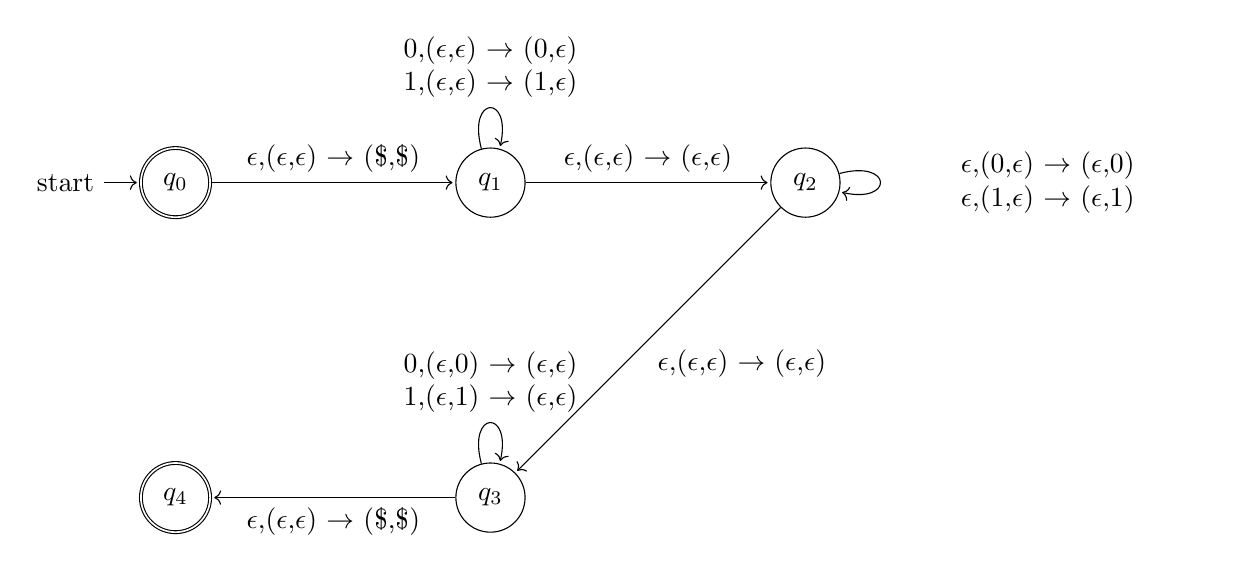
\begin{tikzpicture}[shorten >=1pt,node distance=4cm,on grid,auto] 
        \node[state,initial,accepting]  (q_0)                   {$q_0$}; 
        \node[state]  					(q_1)   [right=of q_0]  {$q_1$}; 
        \node[state]            		(q_2)   [right=of q_1]  {$q_2$};
		\node[state]            		(q_3)   [below=of q_1]  	{$q_3$};
		\node[state,accepting]     		(q_4)   [below=of q_0]  	{$q_4$};         
        \path[->]
        (q_0)   edge                    node {$\epsilon$,($\epsilon$,$\epsilon$) $\rightarrow$ 											 (\$,\$) }        			   	(q_1)
        (q_1)	edge	[loop above]	node [text width=4cm,align=center]
        									 {0,($\epsilon$,$\epsilon$) $\rightarrow$ (0,$													 \epsilon$)\\
        									  1,($\epsilon$,$\epsilon$) $\rightarrow$ (1,$													 \epsilon$)}
        (q_1)   edge                    node {$\epsilon$,($\epsilon$,$\epsilon$) $\rightarrow$ 											 ($\epsilon$,$\epsilon$)}      	(q_2)
        (q_2)   edge    [loop right]    node [text width=4cm,align=center]
        									 {$\epsilon$,(0,$\epsilon$) $\rightarrow$ ($													 \epsilon$,0)\\
        									  $\epsilon$,(1,$\epsilon$) $\rightarrow$ ($													 \epsilon$,1)}					(q_2)
		(q_2)   edge                    node {$\epsilon$,($\epsilon$,$\epsilon$) $\rightarrow$ 											 ($\epsilon$,$\epsilon$)}      	(q_3)
		(q_3)	edge	[loop above]	node [text width=4cm,align=center]
        									 {0,($\epsilon$,0) $\rightarrow$ ($\epsilon$,$													 \epsilon$)\\
        									  1,($\epsilon$,1) $\rightarrow$ ($\epsilon$,$													 \epsilon$)}					(q_3)
		(q_3)   edge                    node {$\epsilon$,($\epsilon$,$\epsilon$) $\rightarrow$ 											 (\$,\$)}      					(q_4)
		
        ; %end path 
    \end{tikzpicture}

\pagebreak

\section*{3.}
wx $\epsilon$ A and x $\epsilon$ B. w is CFL and x is regular so A$\diagdown$B means that A is still CFL because x is excluded.
\includegraphics[scale=0.6]{mynd}


\section*{4.}

\textbf{PDA:}\\
    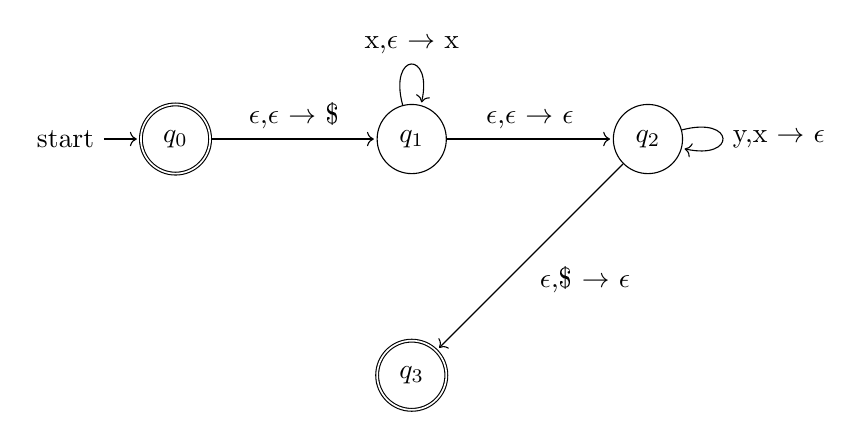
\begin{tikzpicture}[shorten >=1pt,node distance=3cm,on grid,auto] 
        \node[state,initial,accepting]  (q_0)                   {$q_0$}; 
        \node[state]  					(q_1)   [right=of q_0]  {$q_1$}; 
        \node[state]            		(q_2)   [right=of q_1]  {$q_2$};         
		\node[state,accepting]     		(q_3)   [below=of q_1]  {$q_3$};        
        \path[->]
        (q_0)   edge                    node {$\epsilon$,$\epsilon$ $\rightarrow$ \$} (q_1)
        (q_1)	edge	[loop above]	node [text width=4cm,align=center]
        									 {x,$\epsilon$ $\rightarrow$ x}
        (q_1)   edge                    node {$\epsilon$,$\epsilon$ $\rightarrow$ 															 $\epsilon$}      	(q_2)
        (q_2)   edge    [loop right]    node {y,x $\rightarrow$ $\epsilon$} (q_2)
        (q_2)	edge					node {$\epsilon$,\$ $\rightarrow$ $\epsilon$}		(q_3)
		
        ; %end path 
    \end{tikzpicture}

\pagebreak

\section*{5.}
\subsection*{a)}

\textbf{PDA:}\\
    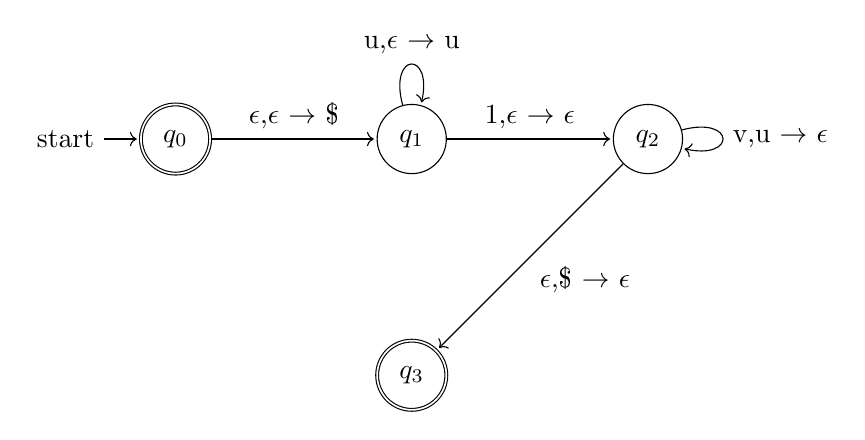
\begin{tikzpicture}[shorten >=1pt,node distance=3cm,on grid,auto] 
        \node[state,initial,accepting]  (q_0)                   {$q_0$}; 
        \node[state]  					(q_1)   [right=of q_0]  {$q_1$}; 
        \node[state]            		(q_2)   [right=of q_1]  {$q_2$};         
		\node[state,accepting]     		(q_3)   [below=of q_1]  {$q_3$};        
        \path[->]
        (q_0)   edge                    node {$\epsilon$,$\epsilon$ $\rightarrow$ \$} (q_1)
        (q_1)	edge	[loop above]	node [text width=4cm,align=center]
        									 {u,$\epsilon$ $\rightarrow$ u}
        (q_1)   edge                    node {1,$\epsilon$ $\rightarrow$ $\epsilon$}  (q_2)
        (q_2)   edge    [loop right]    node {v,u $\rightarrow$ $\epsilon$} (q_2)
        (q_2)	edge					node {$\epsilon$,\$ $\rightarrow$ $\epsilon$} (q_3)
	
		; %end path 
    \end{tikzpicture}


\subsection*{b)}


\end{document}